\section{Rewrite Rules}

This section introduces the various rewrite rules that come equipped with the ZX calculus. These rules extend the ZX calculus from notation into a language.

\subsection{Spider Fusion}%
\label{spider-fusion}

The most fundamental rule of the ZX calculus is the \textit{spider fusion} rule \cite{Wetering2020}. It states that two spiders connected by one or more wires fuse if they are the same colour. It is the generalisation of adding the phases of successive rotations of the Bloch sphere. Since we interpret the phases $\alpha$ and $\beta$ as $e^{i\alpha}$ and $e^{i\beta}$, it follows that the phase $\alpha + \beta$ is modulo $2\pi$.

\begin{figure}[H]
    \centering
    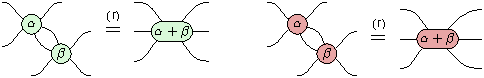
\includegraphics[width=0.8\textwidth]{chapter-2/fusion}
    \caption{Spider fusion rule for $Z$ spiders (left) and $X$ spiders (right).}
\end{figure}

We can use this rule to identify commutation relations. For instance, $Z$ rotations commute through CNOT controls and $X$ rotations commute through CNOT targets.

% \vspace{5pt}
\includezxdiagram{chapter-2/cnot_commutation}{0.9}

%%%

\subsection{Identity Removal}%
\label{identity}

The \textit{identity removal} rule states that any two-legged spider with no phase ($\alpha = 0$) is equivalent to an empty wire since a rotation by 0 radians is the same as no rotation.

\begin{figure}[H]
    \centering
    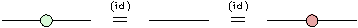
\includegraphics[width=0.65\textwidth]{chapter-2/identity}
    \caption{Identity removal rule.}
\end{figure}

Combining this with the spider fusion rule (\ref{spider-fusion}), we see that two successive rotations with opposite phases is equivalent to an empty wire.

\includezxdiagram{chapter-2/cancelling_rotations}{0.8}

%%%

\subsection{$\pi$ Copy Rule}%
\label{pi-copy}

The $\pi$ \textit{copy} rule concerns itself with the interactions of the Pauli $Z$ and $X$ gates with spiders. It states that when a Pauli $Z$ or Pauli $X$ gate is pushed through a spider of the opposite colour, it copies through the spider and flips its phase.

\begin{figure}[H]
    \centering
    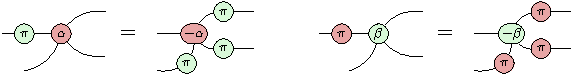
\includegraphics[width=1\textwidth]{chapter-2/pi_copy}
    \caption{$\pi$ copy rule for $Z$ and and $X$ spiders.}
\end{figure}

% The $\pi$ copy rule shows us that the Pauli $Z$ and Pauli $X$ gates interact with states (spiders with no inputs) as follows.
% \includezxdiagram{chapter-2/pi_copy_state}{0.75}

\subsection{State Copy Rule}%
\label{state-copy}

A similar rule derived from the $\pi$ copy rule (\ref{pi-copy}), is the \textit{state copy} rule. It states that the $\ket 0$ state (phaseless $X$ spider) and the $\ket 1$ state ($X$ spider with phase $\pi$) interact with $Z$ spiders as follows. The same rule holds for the colour-flipped counterparts.

\begin{figure}[H]
    \centering
    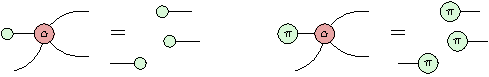
\includegraphics[width=0.9\textwidth]{chapter-2/state_copy}
    \caption{State copy rule for the $X$ eigenstates.}
\end{figure}

%%%

\subsection{Bialgebra Rule}%
\label{bialgebra}
Unlike the previous rules we have introduced, the \textit{bialgebra rule} takes some time to understand intuitively. It is nethertheless important in many derivations. We can represent the eigenstates of the $X$ and $Z$ operators by introducing the boolean variable $a \in \{0, 1\}$ as follows.

\begin{center}
\includezxdiagramtext{chapter-2/boolean_x}{0.085}{
\ket 0 \text{ where $a = 0$ and }
\ket 1 \text{ where $a = 1$}}
\includezxdiagramtext{chapter-2/boolean_z}{0.085}{
\ket + \text{ where $a = 0$ and }
\ket - \text{ where $a = 1$}}
\end{center}

Using the spider fusion rule (\ref{spider-fusion}), we are able to show that an $X$ spider with two inputs and one output behaves like the classical XOR gate when applied to the $\ket 0$ and $\ket 1$ states. Using the state copy rule (\ref{state-copy}), we are able to show that a $Z$ spider with one input and two outputs behaves like the classical COPY gate.

\begin{figure}[H]
    \centering
    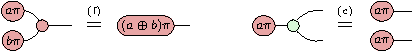
\includegraphics[width=0.77\textwidth]{chapter-2/xor_copy}
    \caption{$X$ spider as a XOR gate (left) and $Z$ spider as a COPY gate (right).}
\end{figure}

Let us now consider the natural commutation relation of the classical XOR and COPY gates. It is clear that XORing two bits then copying them is the same as copying the same two bits, then XORing them. Using this relation as motivation, we define the \textit{bialgebra} rule.

\begin{figure}[H]
    \centering
    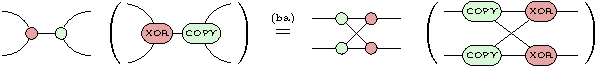
\includegraphics[width=0.7\textwidth]{chapter-2/bialgebra}
    \caption{The bialgebra rule (top) and its classical motivation (bottom).}
\end{figure}

The bialgebra rule is then the quantum generalisation of the XOR-COPY commutation relation. It holds for all states, not just the computational basis states.

%%%

\subsection{Hopf Rule}%
\label{hopf}

Finally, we have the Hopf rule, which states that we can remove the wires connecting an $X$ spider and a $Z$ spider when the number of connections between them is two. Like with the bialgebra rule (\ref{bialgebra}), we can take motivation from the behaviour of the classical XOR and COPY gates, since COPYing two bits then XORing them always yields 0.

\begin{figure}[H]
    \centering
    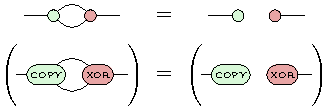
\includegraphics[width=0.7\textwidth]{chapter-2/hopf}
    \caption{The Hopf rule (top) and its classical motivation (bottom).}
\end{figure}

